%!TEX root = ../these.tex

\subsection*{%
Решение задач большой размерности
}
\label{sec:ccp.ufa}

Интересно сравнить решения,
полученные в~Главе~\ref{ch:pcgtsp}
(см. рис.~\ref{fig:pcgtsp.ufa}
на стр.~\pageref{fig:pcgtsp.ufa})
с решениями задачи непрерывной резки
для тех же раскройных планов,
содержащих сотни контуров.

Решения,
не использующие механизм дискретизации,
приведены на
рис.~\ref{fig:ccp.ufa},
численные данные ---
в~табл.~\ref{tab:ccp.ufa}.

\begin{table}[h]
  \centering
  \caption{Результаты решения задач CCP большой размерности}
  \label{tab:ccp.ufa}
  \begin{tabular}{*{4}{|r}|}
    \hline
    Деталей & Контуров & Вложенность & $\mathcal L$, мм \\
    \hline
    125 & 423 & 6 & 22609 \\
    140 & 620 & 2 & 32051 \\
    \hline
  \end{tabular}
\end{table}

Несмотря на то,
что решения разных задач
нельзя сравнивать напрямую,
тем не менее
полезно сравнить их,
особенно с учетом того,
что для задач такой размерности
пока невозможно точно судить об оптимальности решения.
Очевидное сходство решений,
полученных разными методами
позволяет осторожно предполагать,
близость обоих решений к оптимальным
для своего класса задач.
Как и в более простых примерах,
решения задачи CCP
оказываются чуть лучше,
чем решения задачи PCGTSP,
но разница становится больше и
на приведенных примерах достигает
$\approx 8\%$,
что отчасти объясняется тем,
что на рис.~\ref{fig:pcgtsp.ufa}
применялась более грубая
дискретизация
(ввиду большего размера задачи).

\begin{figure}
  \centering
  \subfloat[125 деталей; 423 контура]{
    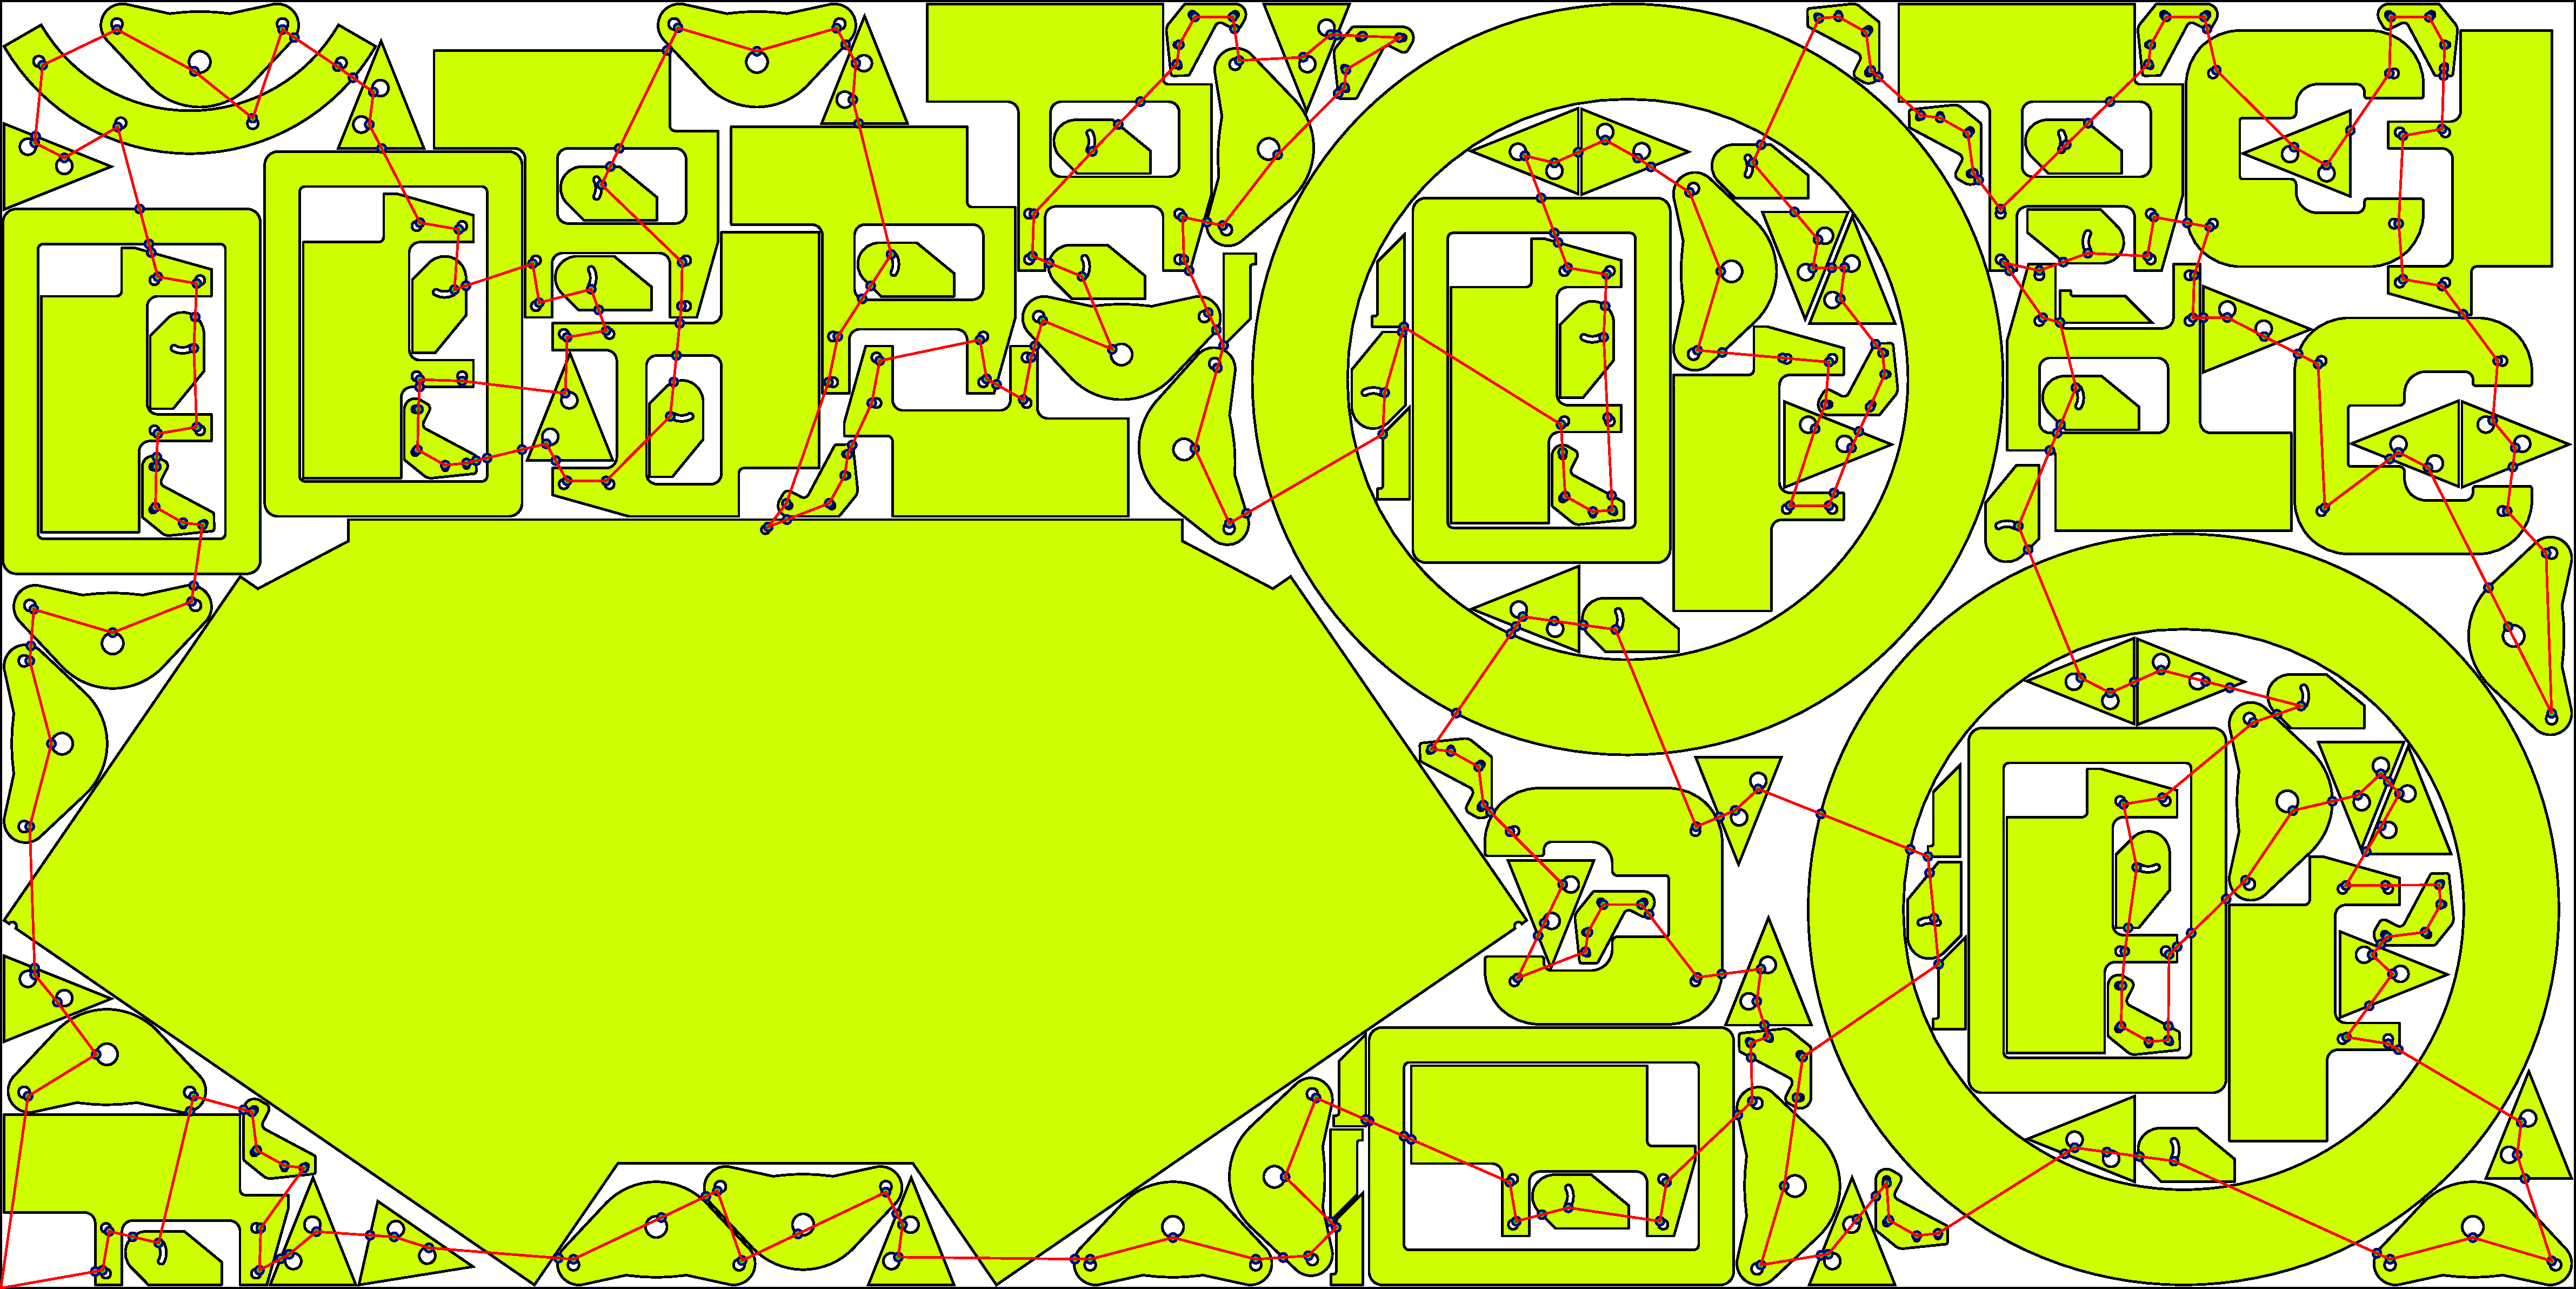
\includegraphics[width=0.95\textwidth]{ufa/a.ccp.pdf}
  }
  \\
  \subfloat[140 деталей; 620 контуров]{
    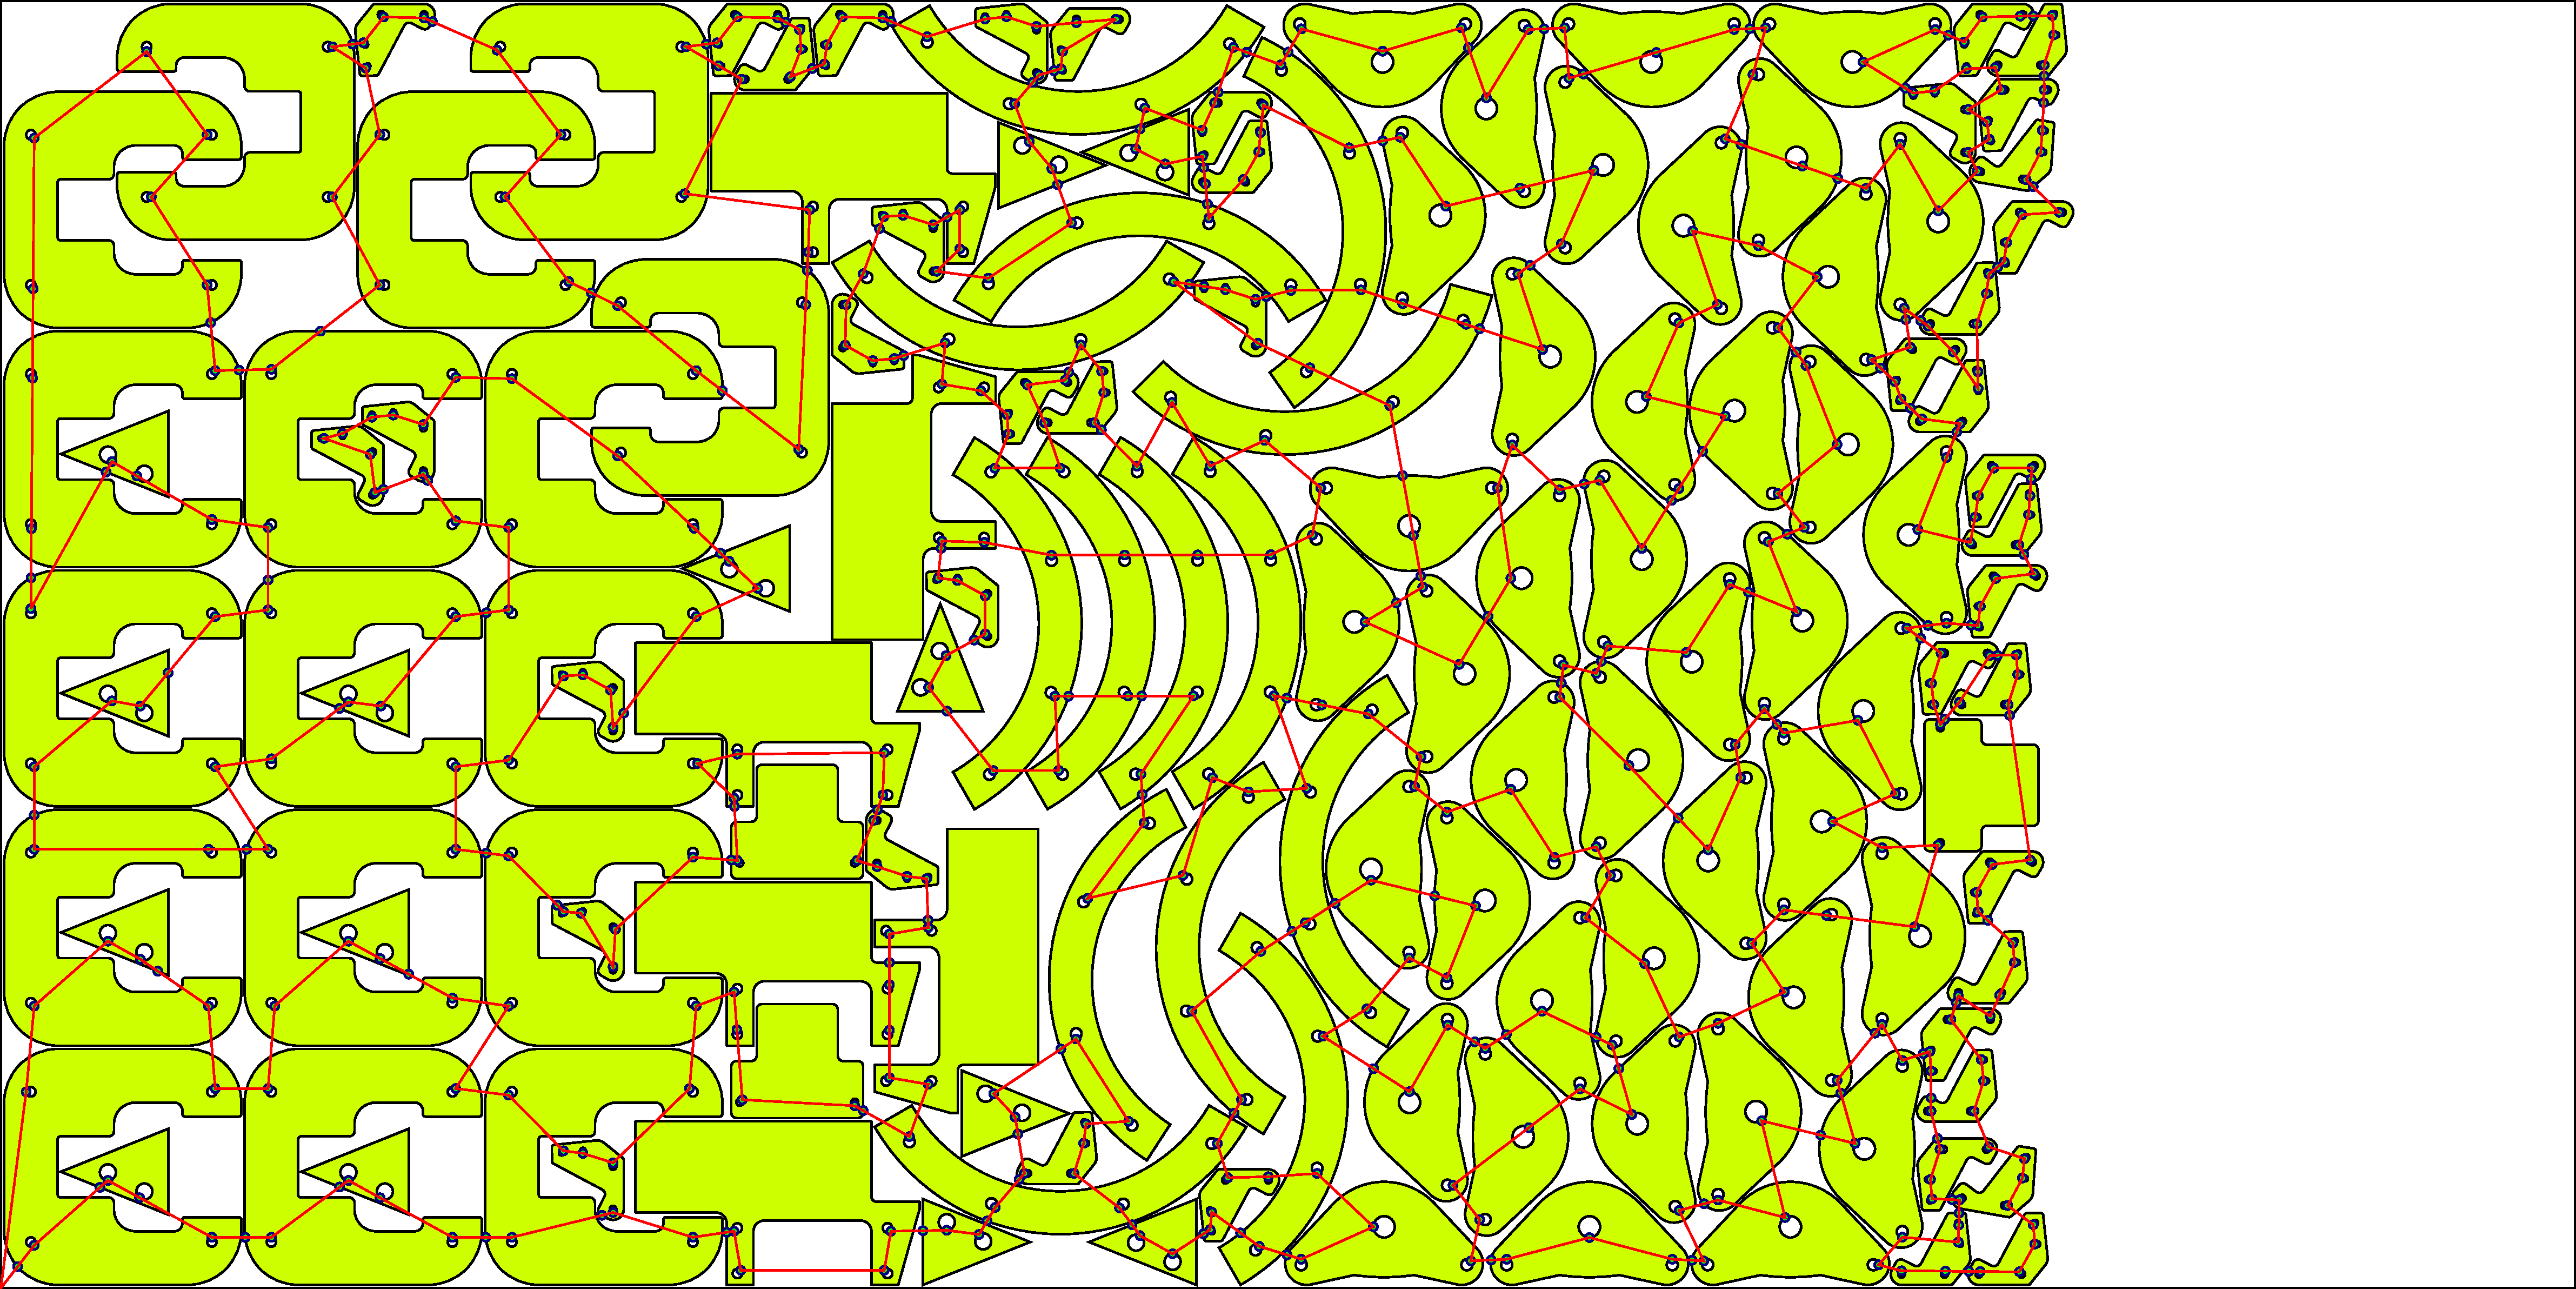
\includegraphics[width=0.95\textwidth]{ufa/b.ccp.pdf}
  }
  \caption{Решения задач CCP большой размерности}
  \label{fig:ccp.ufa}
\end{figure}

